\documentclass[11pt]{article}
\usepackage[margin=0.9in]{geometry}
\usepackage{amsmath,amssymb}
\usepackage{booktabs}
\usepackage{graphicx}
\usepackage{fancyhdr}
\usepackage[hidelinks]{hyperref}

\graphicspath{{Figures/}}
\pagestyle{fancy}
\fancyhf{}
\lhead{STAT 546 \textbar{} HW6 implementation report \textbar{} Anurag Ramesh}
\rhead{6 November 2026}
\cfoot{\thepage}
\renewcommand{\headrulewidth}{0.4pt}
\setlength{\headheight}{14pt}
\setlength{\parindent}{0pt}
\setlength{\parskip}{6pt}

\newcommand{\E}{\mathbb{E}}
\DeclareMathOperator*{\argmin}{arg\,min}

\begin{document}

All code is in \texttt{Scripts/}, one script per computational question (Q1, Q2 and Q4). The general methods
are in the root modules \path{Stochastic_Approximation.py} and \path{Expectation_Maximization.py}. Each
script saves its figure in \texttt{Figures/} and its numbers in \texttt{Results/}. Q3 and Q5 are derivations.

\section*{Q1. Robbins--Monro for the root of $\E(X-\theta)=0$}

With $X\sim N(\mu,\sigma^2)$, $h(\theta)=\E(X-\theta)=\mu-\theta$, so the root is $\theta^*=\mu$. Robbins and
Monro (1951) replace the unknown $h$ by one noisy evaluation per step:
\[
\theta_k=\theta_{k-1}+a_k\,(X_k-\theta_{k-1}),\qquad k=1,2,\ldots,
\]
with $X_1,X_2,\ldots$ independent draws. I used $\mu=5$, $\sigma=2$ and $\theta_0=0$.

\subsection*{Exact mean squared error}

Because $h$ is linear, the error $e_k=\theta_k-\mu$ satisfies
$e_k=(1-a_k)e_{k-1}+a_k\varepsilon_k$, where $\varepsilon_k=X_k-\mu\sim N(0,\sigma^2)$ is independent of
$e_{k-1}$. Squaring and taking expectations gives the exact recursion
\[
\mathrm{MSE}_k=(1-a_k)^2\,\mathrm{MSE}_{k-1}+a_k^2\sigma^2,\qquad \mathrm{MSE}_0=(\theta_0-\mu)^2.
\]
Its long-run behaviour depends on the schedule:
\begin{itemize}
\item $a_k=1/k$: then $\theta_k=\frac1k\sum_{j\le k}X_j$, the sample mean, and $\mathrm{MSE}_k=\sigma^2/k$
exactly for $k\ge1$.
\item $a_k=a/k$ with $a>\tfrac12$: trying $\mathrm{MSE}_k\approx c/k$ in the recursion gives
$c=a^2\sigma^2/(2a-1)$. This is never below $\sigma^2$, the value at $a=1$; for $a=2$ it is
$\tfrac43\sigma^2$.
\item $a_k=a/k$ with $a<\tfrac12$: the error shrinks only by $\prod_{j\le k}(1-a/j)\approx k^{-a}$, and
$\mathrm{MSE}_k$ decays like $k^{-2a}$, slower than $1/k$.
\item $a_k=k^{-\alpha}$ with $\tfrac12<\alpha<1$: the error tracks a slowly moving balance,
$\mathrm{MSE}_k\approx a_k\sigma^2/2$, which decays like $k^{-\alpha}$.
\item $a_k=a$ constant: the recursion has the fixed point $a\sigma^2/(2-a)$, so $\theta_k$ keeps fluctuating
and never converges.
\end{itemize}
The first four schedules satisfy the Robbins--Monro conditions $\sum_k a_k=\infty$ and $\sum_k a_k^2<\infty$;
the constant step violates the second.

\subsection*{Results}

I ran 1,000 independent replicates of 10,000 steps for each schedule (seed 546). The table compares the
simulated mean squared error with the exact recursion.

\begin{center}
\begin{tabular}{lcccccc}
\toprule
& \multicolumn{2}{c}{$k=100$} & \multicolumn{2}{c}{$k=1{,}000$} & \multicolumn{2}{c}{$k=10{,}000$} \\
\cmidrule(lr){2-3}\cmidrule(lr){4-5}\cmidrule(lr){6-7}
\textbf{Schedule} & Simulated & Exact & Simulated & Exact & Simulated & Exact \\
\midrule
$a_k=1/k$ & 0.0365 & 0.0400 & 0.00409 & 0.00400 & 0.000400 & 0.000400 \\
$a_k=0.2/k$ & 2.978 & 2.979 & 1.187 & 1.188 & 0.4728 & 0.4733 \\
$a_k=2/k$ & 0.0557 & 0.0536 & 0.00544 & 0.00534 & 0.000523 & 0.000533 \\
$a_k=k^{-0.6}$ & 0.131 & 0.137 & 0.0306 & 0.0326 & 0.00794 & 0.00804 \\
$a_k=0.05$ & 0.110 & 0.103 & 0.0949 & 0.1026 & 0.0986 & 0.1026 \\
\bottomrule
\end{tabular}
\end{center}

The simulations agree with the exact recursion, and the schedules behave as derived. $a_k=1/k$ is best. $a_k=2/k$
has the same $1/k$ rate with a constant $4/3$ times larger. $a_k=0.2/k$ moves so slowly that after 10,000 steps
the error is still about 0.69 in root mean square. $a_k=k^{-0.6}$ converges at the slower rate $k^{-0.6}$.
The constant step approaches the root quickly at first but then stays at a mean squared error of about $0.10$.

\begin{center}
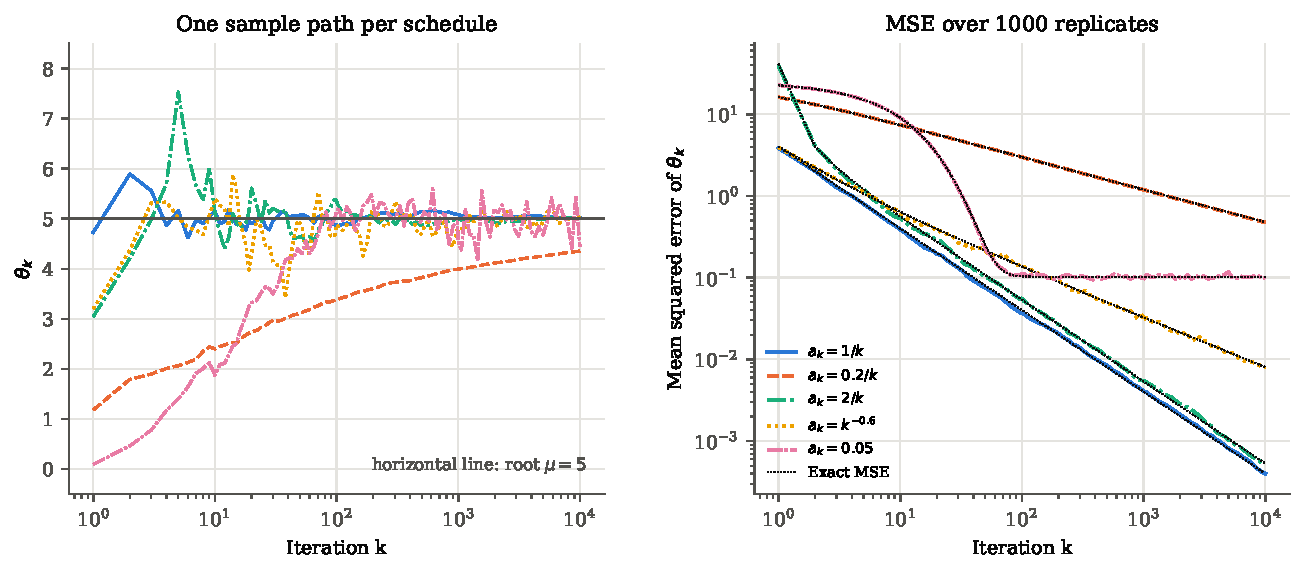
\includegraphics[width=\textwidth]{q1_robbins_monro.pdf}
\end{center}

\newpage
\section*{Q2. Minibatch SGD for logistic regression}

\subsection*{Model and update}

For $Y_i\in\{0,1\}$ and $P(Y_i=1\mid x_i)=s(x_i^T\theta)$ with $s(z)=1/(1+e^{-z})$, the log-likelihood of one
observation and its gradient are
\[
\ell_i(\theta)=Y_ix_i^T\theta-\log\left(1+e^{x_i^T\theta}\right),\qquad
\nabla\ell_i(\theta)=\left(Y_i-s(x_i^T\theta)\right)x_i .
\]
The training loss is $L(\theta)=-\frac1n\sum_i\ell_i(\theta)$. Each epoch shuffles the training set and splits it
into minibatches $B$ of size $b$; for each minibatch,
\[
\theta\leftarrow\theta+\eta_t\,\frac{1}{|B|}\sum_{i\in B}\left(Y_i-s(x_i^T\theta)\right)x_i ,
\qquad \eta_t=\eta_0\left(1+t/T\right)^{-p},
\]
where $t$ counts updates and $T=\lceil n/b\rceil$ is the number of updates per epoch, so $p=0$ is a constant
rate and $p>0$ decays it by epoch.

\subsection*{Data and settings}

I simulated an intercept and 20 independent $N(0,1)$ predictors, with intercept $-0.5$, coefficients
$\pm1$ for predictors 1--5, $\pm0.5$ for predictors 6--10 (alternating signs) and 0 for the rest. The training
and test sets have 10,000 observations each (data seed 546; SGD seed 547). Every run starts at $\theta=0$ and
lasts 30 epochs. The baseline is $b=32$, $\eta_0=0.1$, $p=0$, and each comparison changes one factor. The
decay comparison uses $\eta_0=1$, so that decay has a large constant rate to correct.

Two reference values come from the same data. The minimum training loss, from an unpenalized maximum
likelihood fit, is 0.40159. The test error of the true coefficients is 0.1814 (0.1828 for the maximum
likelihood fit). Test error is the misclassification rate of the rule $x^T\theta>0$.

\subsection*{Results after 30 epochs}

\begin{center}
\begin{tabular}{llcc}
\toprule
\textbf{Comparison} & \textbf{Setting} & \textbf{Training loss minus minimum} & \textbf{Test error} \\
\midrule
Batch size ($\eta_0=0.1$, $p=0$) & $b=1$ & $8.8\times10^{-2}$ & 0.2111 \\
 & $b=8$ & $6.3\times10^{-3}$ & 0.1839 \\
 & $b=64$ & $4.5\times10^{-4}$ & 0.1824 \\
 & $b=512$ & $2.3\times10^{-4}$ & 0.1831 \\
\midrule
Learning rate ($b=32$, $p=0$) & $\eta_0=0.01$ & $1.9\times10^{-5}$ & 0.1829 \\
 & $\eta_0=0.1$ & $1.2\times10^{-3}$ & 0.1839 \\
 & $\eta_0=1$ & $3.2\times10^{-2}$ & 0.1966 \\
 & $\eta_0=5$ & $3.2\times10^{-1}$ & 0.2527 \\
\midrule
Decay ($b=32$, $\eta_0=1$) & $p=0$ & $3.2\times10^{-2}$ & 0.1966 \\
 & $p=0.5$ & $2.8\times10^{-3}$ & 0.1843 \\
 & $p=1$ & $1.0\times10^{-4}$ & 0.1829 \\
\bottomrule
\end{tabular}
\end{center}

\textbf{Batch size.} With a fixed rate, small batches give noisy gradients, and the training loss stops falling
at a level set by that noise: $b=1$ stays about 0.09 above the minimum. Larger batches average out the noise but
make fewer updates per epoch; $b=512$ makes only 20 updates per epoch, so its loss falls slowly but steadily.

\textbf{Learning rate.} A larger constant rate reduces the loss faster at first but leaves a higher noise
plateau. $\eta_0=5$ never settles, and its test error jumps between 0.21 and 0.32. $\eta_0=0.01$ is still
improving at epoch 30 and reaches the smallest loss here.

\textbf{Decay.} With $\eta_0=1$, a constant rate plateaus at 0.03 above the minimum. Decaying the rate keeps the
fast start but removes the plateau; $p=1$ ends $10^{-4}$ above the minimum.

Test error changes much less than training loss. At epoch 30, every run whose loss is within $10^{-2}$ of its
minimum has test error within 0.003 of that of the true coefficients.

\begin{center}
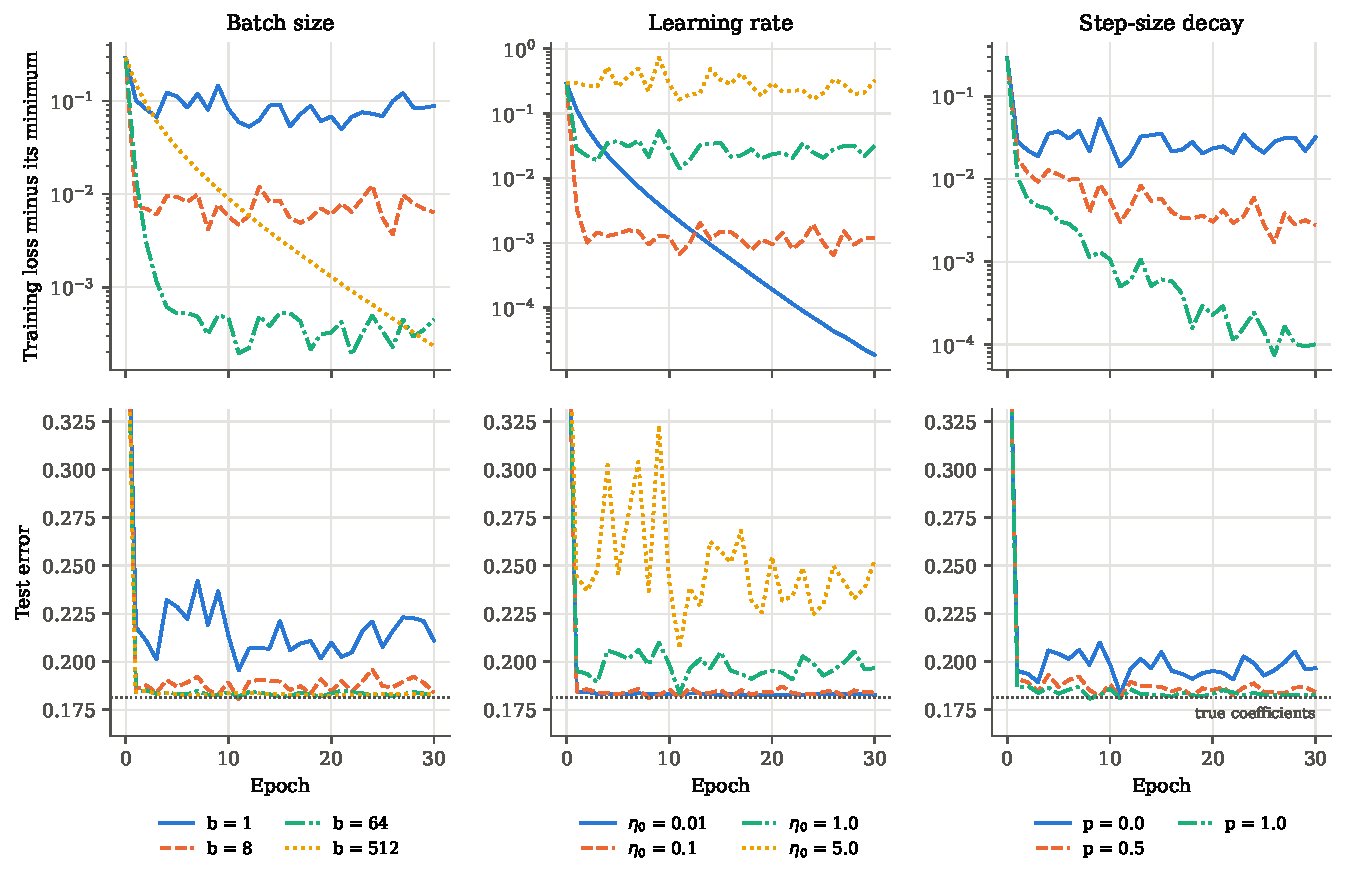
\includegraphics[width=\textwidth]{q2_sgd_logistic.pdf}
\end{center}

These comparisons come from one simulated dataset and one SGD seed.

\newpage
\section*{Q3. SGD for the penalized empirical risk}

Here $\ell(Y_i,X_i;\theta)$ is the log-likelihood of observation $i$, written $\ell_i(\theta)$. The penalized
empirical risk and its gradient are
\[
U(\theta)=-\frac1n\sum_{i=1}^n\ell_i(\theta)+\lambda\|\theta\|_2^2,
\qquad
\nabla U(\theta)=-\frac1n\sum_{i=1}^n\nabla\ell_i(\theta)+2\lambda\theta .
\]
At step $t$, draw a minibatch $B_t$ of size $b$ uniformly at random from $\{1,\ldots,n\}$. The stochastic
gradient
\[
\hat g_t=-\frac1b\sum_{i\in B_t}\nabla\ell_i(\theta_t)+2\lambda\theta_t
\]
is unbiased, $\E[\hat g_t\mid\theta_t]=\nabla U(\theta_t)$, because each observation is equally likely to be in
$B_t$. The SGD update $\theta_{t+1}=\theta_t-\eta_t\hat g_t$ is therefore
\[
\boxed{\;\theta_{t+1}=(1-2\eta_t\lambda)\,\theta_t+\eta_t\,\frac1b\sum_{i\in B_t}\nabla\ell_i(\theta_t)\;}
\]
For logistic regression, $\nabla\ell_i(\theta)=(Y_i-s(x_i^T\theta))x_i$, as in Q2. With $\lambda=0$ this is the
Q2 update. The function \texttt{sgd\_logistic\_regression} implements it through its \texttt{lam} argument, and
a test checks one step against this formula.

\subsection*{How the penalty changes the update}

\begin{itemize}
\item \textbf{Shrinkage (weight decay).} Before the data step, every step multiplies $\theta_t$ by
$1-2\eta_t\lambda$, pulling all coefficients toward zero. Without the data term, $\theta$ would decay
geometrically to 0.
\item \textbf{No extra noise.} The penalty gradient $2\lambda\theta_t$ is computed exactly, not estimated from
the minibatch. All randomness in $\hat g_t$ comes from the data term, so the penalty adds bias toward zero but no
variance.
\item \textbf{A restriction on the step size.} The factor $1-2\eta_t\lambda$ must stay in $(0,1)$, that is
$\eta_t<1/(2\lambda)$. Otherwise the shrinkage overshoots and changes the sign of $\theta$.
\item \textbf{A different target.} SGD is the Robbins--Monro algorithm of Q1 applied to $h(\theta)=-\nabla U(\theta)$.
Its root is the penalized estimate $\hat\theta_\lambda$, where the data gradient no longer vanishes but balances
the shrinkage:
\[
\frac1n\sum_{i=1}^n\nabla\ell_i(\hat\theta_\lambda)=2\lambda\hat\theta_\lambda .
\]
\item \textbf{Better behaviour of the target.} When $-\ell_i$ is convex, as in logistic regression, the penalty
makes $U$ strongly convex with constant $2\lambda$, so $\hat\theta_\lambda$ exists and is unique. For logistic
regression this holds even when the classes are perfectly separable, where the unpenalized estimate does not
exist.
\end{itemize}

\newpage
\section*{Q4. EM for a finite mixture of univariate normals}

\subsection*{Derivation}

The model is $f(x)=\sum_{k=1}^K\pi_k\,\phi(x;\mu_k,\sigma_k^2)$, with $\phi$ the normal density and
$\theta=(\pi_k,\mu_k,\sigma_k^2)_{k=1}^K$. The observed-data log-likelihood is
\[
\ell(\theta)=\sum_{i=1}^n\log\sum_{k=1}^K\pi_k\,\phi(x_i;\mu_k,\sigma_k^2).
\]
Let $z_{ik}=1$ if observation $i$ comes from component $k$ and 0 otherwise. If the $z_{ik}$ were known, the
complete-data log-likelihood would be
\[
\ell_c(\theta)=\sum_{i=1}^n\sum_{k=1}^K z_{ik}\left[\log\pi_k-\tfrac12\log(2\pi\sigma_k^2)
-\frac{(x_i-\mu_k)^2}{2\sigma_k^2}\right].
\]

\textbf{E-step.} $\ell_c$ is linear in $z_{ik}$, so its conditional expectation given the data and the current
estimate $\theta^{(t)}$ replaces $z_{ik}$ by
\[
r_{ik}^{(t)}=P(z_{ik}=1\mid x_i,\theta^{(t)})
=\frac{\pi_k^{(t)}\phi(x_i;\mu_k^{(t)},\sigma_k^{2(t)})}{\sum_{j=1}^K\pi_j^{(t)}\phi(x_i;\mu_j^{(t)},\sigma_j^{2(t)})}
\]
by Bayes' rule, giving
$Q(\theta\mid\theta^{(t)})=\sum_i\sum_k r_{ik}^{(t)}\left[\log\pi_k-\tfrac12\log(2\pi\sigma_k^2)
-(x_i-\mu_k)^2/(2\sigma_k^2)\right]$.

\textbf{M-step.} Write $n_k=\sum_i r_{ik}^{(t)}$. For the weights, maximize $\sum_k n_k\log\pi_k$ subject to
$\sum_k\pi_k=1$. The Lagrangian condition $n_k/\pi_k=\nu$ and the constraint give $\nu=n$. For each mean and
variance, set the partial derivatives of $Q$ to zero:
\[
\frac{\partial Q}{\partial\mu_k}=\sum_i r_{ik}^{(t)}\frac{x_i-\mu_k}{\sigma_k^2}=0,
\qquad
\frac{\partial Q}{\partial\sigma_k^2}=\sum_i r_{ik}^{(t)}\left[-\frac{1}{2\sigma_k^2}+\frac{(x_i-\mu_k)^2}{2\sigma_k^4}\right]=0 .
\]
The updates are therefore
\[
\pi_k^{(t+1)}=\frac{n_k}{n},\qquad
\mu_k^{(t+1)}=\frac{\sum_i r_{ik}^{(t)}x_i}{n_k},\qquad
\sigma_k^{2(t+1)}=\frac{\sum_i r_{ik}^{(t)}\left(x_i-\mu_k^{(t+1)}\right)^2}{n_k}.
\]
These are weighted versions of the sample proportion, mean and variance, with observation $i$ given weight
$r_{ik}^{(t)}$ in component $k$.

\textbf{Monotone log-likelihood.} Since $P(z_{ik}=1\mid x_i,\theta)=\pi_k\phi(x_i;\mu_k,\sigma_k^2)/f(x_i)$ and
$\sum_k r_{ik}^{(t)}=1$, the log-likelihood splits as
\[
\ell(\theta)=Q(\theta\mid\theta^{(t)})-H(\theta\mid\theta^{(t)}),\qquad
H(\theta\mid\theta^{(t)})=\sum_{i=1}^n\sum_{k=1}^K r_{ik}^{(t)}\log P(z_{ik}=1\mid x_i,\theta).
\]
By Gibbs' inequality, $H(\theta\mid\theta^{(t)})\le H(\theta^{(t)}\mid\theta^{(t)})$ for every $\theta$, and the
M-step maximizes $Q(\cdot\mid\theta^{(t)})$. Together,
\[
\ell(\theta^{(t+1)})-\ell(\theta^{(t)})\ \ge\ Q(\theta^{(t+1)}\mid\theta^{(t)})-Q(\theta^{(t)}\mid\theta^{(t)})\ \ge\ 0
\]
(Dempster, Laird and Rubin, 1977).

\subsection*{Implementation and data}

Densities and responsibilities are computed with logarithms (log-sum-exp), so small densities do not underflow.
The likelihood is unbounded if a variance shrinks to 0 at one data point, so variances are kept at least
$10^{-8}$ times the sample variance; this floor was never reached. Iteration stops when the log-likelihood
increases by less than $10^{-12}(1+|\ell|)$. Components are reported in order of their means.

I simulated $n=1{,}000$ observations from $0.3\,N(-2,0.7^2)+0.5\,N(1,1)+0.2\,N(5,1.5^2)$ (seed 546) and ran EM
with $K=3$ from 10 random starts: equal weights, means at three distinct random data points, and every variance
equal to the sample variance.

\subsection*{Results}

\begin{center}
\begin{tabular}{lcccccc}
\toprule
& \multicolumn{2}{c}{\textbf{Weight}} & \multicolumn{2}{c}{\textbf{Mean}} & \multicolumn{2}{c}{\textbf{Standard deviation}} \\
\cmidrule(lr){2-3}\cmidrule(lr){4-5}\cmidrule(lr){6-7}
\textbf{Component} & True & EM & True & EM & True & EM \\
\midrule
1 & 0.3 & 0.263 & $-2$ & $-1.999$ & 0.7 & 0.668 \\
2 & 0.5 & 0.552 & 1 & 1.033 & 1.0 & 1.168 \\
3 & 0.2 & 0.186 & 5 & 5.474 & 1.5 & 1.180 \\
\bottomrule
\end{tabular}
\end{center}

The fitted log-likelihood is $-2269.099$, higher than $-2276.375$ at the true parameters, as a maximum
likelihood estimate should be. The differences from the true values reflect sampling variation; the third
component, for example, has only 215 observations.

\textbf{Convergence.} All 10 starts reached the same final log-likelihood, to within $10^{-6}$, after 199 to 403
iterations. The smallest change between iterations, over all starts, was $+2.0\times10^{-9}$, so the
log-likelihood never decreased, as the derivation guarantees. Several starts spend tens to hundreds of
iterations on plateaus near $-2360$ and $-2335$ before rising to the maximum. Near the maximum the distance to the final value
shrinks by a factor of about $0.897$ per iteration. This is linear convergence, and its slow rate is consistent
with the overlap of the first two components, which leaves component membership uncertain for many observations.

\begin{center}
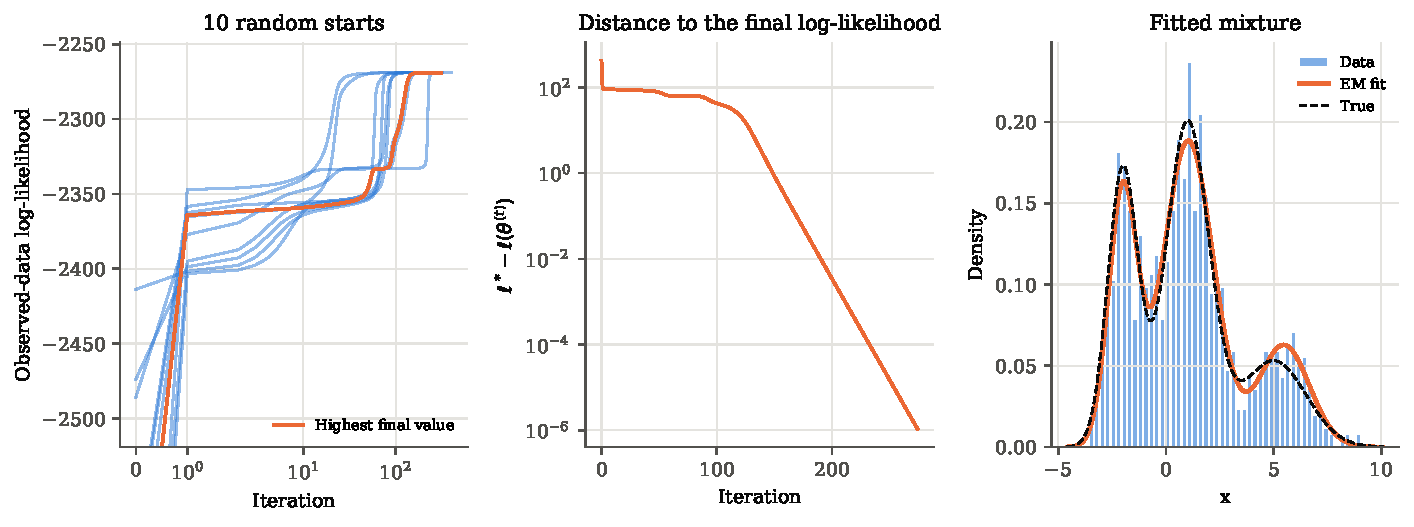
\includegraphics[width=\textwidth]{q4_em_mixture.pdf}
\end{center}

\newpage
\section*{Q5. IRO for regression with covariates missing at random}

\subsection*{Model}

For $i=1,\ldots,n$, let
\[
y_i=\beta_0+x_i^T\beta+\varepsilon_i,\qquad \varepsilon_i\sim N(0,\sigma^2),\qquad x_i\sim N_p(\mu,\Sigma),
\]
with $\Omega=\Sigma^{-1}$, and possibly $p>n$. The responses are fully observed. For each $i$, split the
covariates into observed and missing parts, $x_i=(x_{i,o},x_{i,m})$; the index sets $o$ and $m$ may differ
between observations. The parameter is $\theta=(\beta_0,\beta,\sigma^2,\mu,\Omega)$. A model for $x$ is needed
because the missing values are covariates: they must be drawn from a distribution, which the regression
model alone does not provide.

\textbf{Missing at random.} The probability that an entry is missing may depend on $y_i$ and $x_{i,o}$ but not on
$x_{i,m}$. If the missingness parameters are separate from $\theta$, the mechanism can be ignored, so
\[
f(x_{i,m}\mid x_{i,o},y_i,\text{missingness pattern},\theta)=f(x_{i,m}\mid x_{i,o},y_i,\theta).
\]

\subsection*{Imputation step (I-step)}

Given the current estimate $\theta^{(t)}$, draw the missing covariates of every incomplete observation from their
conditional distribution,
\[
\tilde x_{i,m}^{(t+1)}\sim f(x_{i,m}\mid x_{i,o},y_i,\theta^{(t)})\;\propto\;
f(y_i\mid x_i;\beta_0,\beta,\sigma^2)\,f(x_i;\mu,\Omega).
\]
Up to constants, the logarithm of the right-hand side is
\[
-\tfrac12(x_i-\mu)^T\Omega(x_i-\mu)-\frac{(y_i-\beta_0-x_{i,o}^T\beta_o-x_{i,m}^T\beta_m)^2}{2\sigma^2}.
\]
As a function of $x_{i,m}$ this is quadratic, so the conditional distribution is normal. Collecting the
quadratic and linear terms, with $r_i=y_i-\beta_0-x_{i,o}^T\beta_o$:
\[
x_{i,m}\mid x_{i,o},y_i,\theta\sim N\!\left(\Lambda_i^{-1}b_i,\;\Lambda_i^{-1}\right),\qquad
\Lambda_i=\Omega_{mm}+\frac{\beta_m\beta_m^T}{\sigma^2},\qquad
b_i=\Omega_{mm}\mu_m-\Omega_{mo}(x_{i,o}-\mu_o)+\frac{\beta_m r_i}{\sigma^2},
\]
with every quantity evaluated at $\theta^{(t)}$. Without $y_i$ this would be the usual conditional normal,
with precision $\Omega_{mm}$. The response adds $\beta_m\beta_m^T/\sigma^2$ to the precision and pulls the
mean toward values that explain the residual $r_i$. A draw is $\Lambda_i^{-1}b_i+L_i^{-T}z$ with
$L_iL_i^T=\Lambda_i$ and $z\sim N(0,I)$. The observed entries are kept, giving a pseudo-complete design
$\tilde X^{(t+1)}$.

\subsection*{Regularized optimization step (RO-step)}

Using the pseudo-complete data $(y,\tilde X^{(t+1)})$, compute regularized estimates that remain consistent when
$p>n$:
\begin{align*}
(\beta_0,\beta)^{(t+1)}&=\argmin_{\beta_0,\beta}\left\{\frac{1}{2n}\left\|y-\beta_0\mathbf 1-\tilde X^{(t+1)}\beta\right\|_2^2
+\lambda_\beta\|\beta\|_1\right\},\\
\sigma^{2(t+1)}&=\frac{\left\|y-\beta_0^{(t+1)}\mathbf 1-\tilde X^{(t+1)}\beta^{(t+1)}\right\|_2^2}{n-\hat s-1},
\qquad \hat s=\#\{j:\beta_j^{(t+1)}\ne0\},\\
\mu^{(t+1)}&=\frac1n\sum_{i=1}^n\tilde x_i^{(t+1)},\\
\Omega^{(t+1)}&=\argmin_{\Omega\succ0}\left\{\operatorname{tr}\!\left(S^{(t+1)}\Omega\right)-\log\det\Omega
+\lambda_\Omega\sum_{j\ne k}|\omega_{jk}|\right\},
\end{align*}
where $S^{(t+1)}$ is the sample covariance matrix of $\tilde X^{(t+1)}$. The first line is the Lasso
(Tibshirani, 1996) and the last is the graphical Lasso (Friedman, Hastie and Tibshirani, 2008). The tuning parameters $\lambda_\beta$ and
$\lambda_\Omega$ can be set by cross-validation on the pseudo-complete data, or at rates such as
$\sqrt{\log p/n}$. Other consistent regularized estimators (for example SCAD or MCP for $\beta$, or nodewise
Lasso for $\Omega$) fit the same step.

\subsection*{The algorithm}

\begin{enumerate}
\item \textbf{Start:} fill each missing entry with the mean of the observed values in its column, and apply the
RO-step to obtain $\theta^{(0)}$.
\item \textbf{Iterate} for $t=0,1,\ldots,T-1$: the I-step draws $\tilde X^{(t+1)}$ given $\theta^{(t)}$, and the
RO-step computes $\theta^{(t+1)}$ from $(y,\tilde X^{(t+1)})$.
\item \textbf{Estimate:} because the I-step is random, $\theta^{(0)},\theta^{(1)},\ldots$ form a Markov chain. I
would take the average of $\theta^{(t)}$ after a burn-in period as the final estimate, and the frequency with
which each $\beta_j$ is nonzero after burn-in as a measure of how often it is selected.
\end{enumerate}

IRO (Liang et al., 2018) has the same structure as EM, with two changes that make it workable in high
dimensions. The E-step's expectation over $x_{i,m}$ is replaced by a single draw, so no integral over the missing
values is needed. The M-step's maximum likelihood estimate, which does not exist when $p>n$, is replaced by a
regularized estimate. Liang et al.\ (2018) study the convergence of the resulting iterates.

\newpage
\section*{Saved results}

\texttt{q1.json} contains the simulated and exact mean squared errors. \texttt{q2.json} contains the full
training-loss and test-error curves for every run. \texttt{q4.json} contains the data, the estimates, the final
log-likelihood of every start and the log-likelihood path of the best start.

\section*{References}
\sloppy

STAT 546, Fall 2026. Homework 6, Questions 1--5. The problems and requested methods are taken from the assignment.

H. Robbins and S. Monro (1951). A stochastic approximation method. \emph{The Annals of Mathematical Statistics},
22(3), 400--407. DOI: \href{https://doi.org/10.1214/aoms/1177729586}{10.1214/aoms/1177729586}.

A. P. Dempster, N. M. Laird and D. B. Rubin (1977). Maximum likelihood from incomplete data via the EM algorithm.
\emph{Journal of the Royal Statistical Society, Series B}, 39(1), 1--38.
DOI: \href{https://doi.org/10.2307/2984875}{10.2307/2984875}.

R. Tibshirani (1996). Regression shrinkage and selection via the lasso. \emph{Journal of the Royal Statistical
Society, Series B}, 58(1), 267--288.
DOI: \href{https://doi.org/10.1111/j.2517-6161.1996.tb02080.x}{10.1111/j.2517-6161.1996.tb02080.x}.

J. Friedman, T. Hastie and R. Tibshirani (2008). Sparse inverse covariance estimation with the graphical lasso.
\emph{Biostatistics}, 9(3), 432--441. DOI: \href{https://doi.org/10.1093/biostatistics/kxm045}{10.1093/biostatistics/kxm045}.

F. Liang, B. Jia, J. Xue, Q. Li and Y. Luo (2018). An imputation--regularized optimization algorithm for high
dimensional missing data problems and beyond. \emph{Journal of the Royal Statistical Society, Series B}, 80(5),
899--926. DOI: \href{https://doi.org/10.1111/rssb.12279}{10.1111/rssb.12279}.

\end{document}
